\documentclass[aspectratio=169]{../latex_main/tntbeamer}  % you can pass all options of the beamer class, e.g., 'handout' or 'aspectratio=43'
\usepackage{dsfont}
\usepackage{bm}
\usepackage[english]{babel}
\usepackage[T1]{fontenc}
%\usepackage[utf8]{inputenc}
\usepackage{graphicx}
\graphicspath{ {./figures/} }
\usepackage{algorithm}
\usepackage[ruled,vlined,algo2e,linesnumbered]{algorithm2e}
\usepackage{hyperref}
\usepackage{booktabs}
\usepackage{mathtools}

\usepackage{amsmath,amssymb}

\DeclareMathOperator*{\argmax}{arg\,max}
\DeclareMathOperator*{\argmin}{arg\,min}

\usepackage{pgfplots}
\pgfplotsset{compat=1.16}
\usepackage{tikz}
\usetikzlibrary{trees} 
\usetikzlibrary{shapes.geometric}
\usetikzlibrary{positioning,shapes,shadows,arrows,calc,mindmap}
\usetikzlibrary{positioning,fadings,through}
\usetikzlibrary{decorations.pathreplacing}
\usetikzlibrary{intersections}
\pgfdeclarelayer{background}
\pgfdeclarelayer{foreground}
\pgfsetlayers{background,main,foreground}
\tikzstyle{activity}=[rectangle, draw=black, rounded corners, text centered, text width=8em]
\tikzstyle{data}=[rectangle, draw=black, text centered, text width=8em]
\tikzstyle{myarrow}=[->, thick, draw=black]

% Define the layers to draw the diagram
\pgfdeclarelayer{background}
\pgfdeclarelayer{foreground}
\pgfsetlayers{background,main,foreground}

% Requires XeLaTeX or LuaLaTeX
\usepackage{unicode-math}

\usepackage{fontspec}
%\setsansfont{Arial}
\setsansfont{RotisSansSerifStd}[ 
Path=../latex_main/fonts/,
Extension = .otf,
UprightFont = *-Regular,  % or *-Light
BoldFont = *-ExtraBold,  % or *-Bold
ItalicFont = *-Italic
]
\setmonofont{Cascadia Mono}[
Scale=0.8
]

% scale factor adapted; mathrm font added (Benjamin Spitschan @TNT, 2021-06-01)
%\setmathfont[Scale=1.05]{Libertinus Math}
%\setmathrm[Scale=1.05]{Libertinus Math}

% other available math fonts are (not exhaustive)
% Latin Modern Math
% XITS Math
% Libertinus Math
% Asana Math
% Fira Math
% TeX Gyre Pagella Math
% TeX Gyre Bonum Math
% TeX Gyre Schola Math
% TeX Gyre Termes Math

% Literature References
\newcommand{\lit}[2]{\href{#2}{\footnotesize\color{black!60}[#1]}}

%%% Beamer Customization
%----------------------------------------------------------------------
% (Don't) Show sections in frame header. Options: 'sections', 'sections light', empty
\setbeamertemplate{headline}{empty}

% Add header logo for normal frames
\setheaderimage{
	% 
\includegraphics[height=\logoheight]{figures/TNT_darkv4.pdf}
	
\includegraphics[height=\logoheight]{../latex_main/figures/luh_logo_rgb_0_80_155.pdf}
	% 
\includegraphics[height=\logoheight]{figures/logo_tntluh.pdf}
}

% Header logo for title page
\settitleheaderimage{
	% 
\includegraphics[height=\logoheight]{figures/TNT_darkv4.pdf}
	
\includegraphics[height=\logoheight]{../latex_main/figures/luh_logo_rgb_0_80_155.pdf}
	% 
\includegraphics[height=\logoheight]{figures/logo_tntluh.pdf}
}

% Title page: tntdefault 
\setbeamertemplate{title page}[tntdefault]  % or luhstyle
% Add optional title image here
%\addtitlepageimagedefault{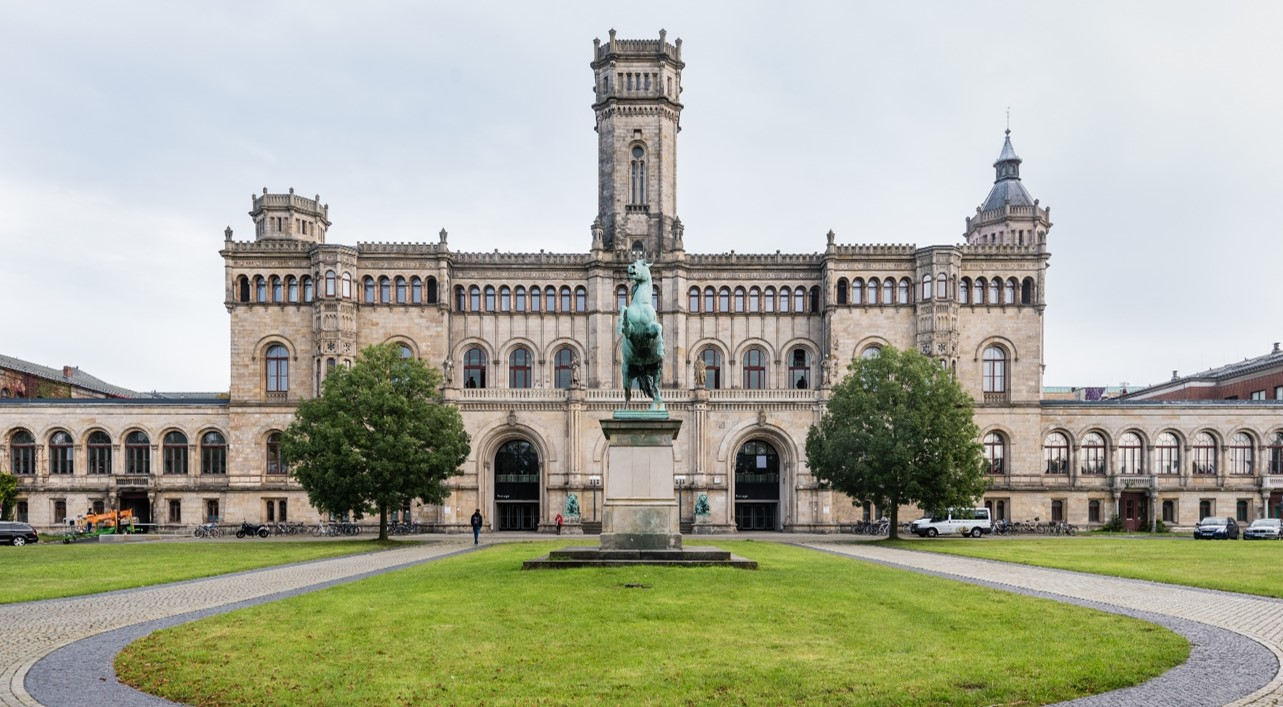
\includegraphics[width=0.65\textwidth]{figures/luh_default_presentation_title_image.jpg}}

% Title page: luhstyle
% \setbeamertemplate{title page}[luhstyle]
% % Add optional title image here
% \addtitlepageimage{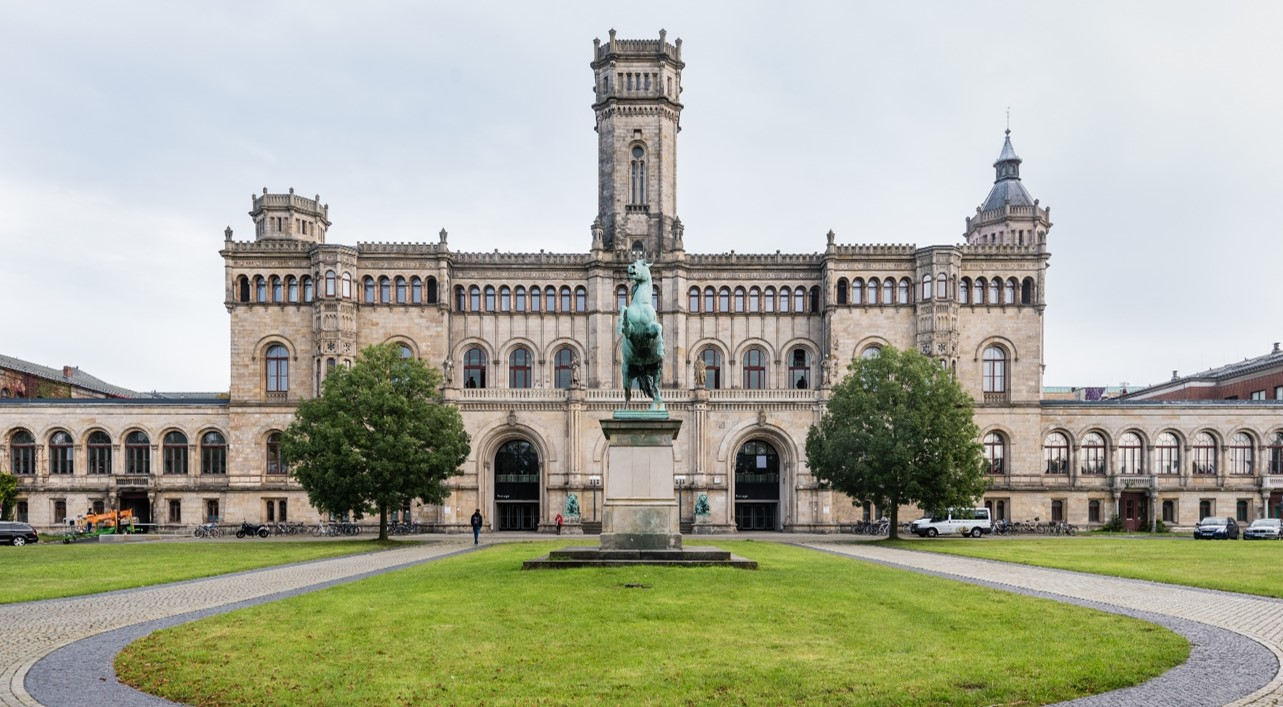
\includegraphics[width=0.75\textwidth]{figures/luh_default_presentation_title_image.jpg}}

\author[Lindauer \& Anand]{Marius Lindauer and Avishek Anand\\[1em]
	
\includegraphics[height=\logoheight]{../latex_main/figures/luh_logo_rgb_0_80_155.pdf}\qquad

\includegraphics[height=\logoheight]{../latex_main/figures/TNT_darkv4}\qquad

\includegraphics[height=\logoheight]{../latex_main/figures/L3S.jpg}	}
\date{Winter Term 2021
}


%%% Custom Packages
%----------------------------------------------------------------------
% Create dummy content
\usepackage{blindtext}

% Adds a frame with the current page layout. Just call \layout inside of a frame.
\usepackage{layout}


\title[Introduction]{iML: Introduction}
\subtitle{fANOVA: Additive Decomposition}
%\institute{}
\newcommand{\predvar}{Var\left[\hat{f}(x)\right]}


\begin{document}
	
	\maketitle

\begin{frame}[c]{High-Dimensional Model Representation}
	
	\begin{itemize}
		\item
		A high-dimensional model representation (HDMR) decomposes the model into a sum of effect terms of increasing order:
		\begin{align*}
		\hat{f}(x) &= g_{\{0\}} + g_{\{1\}}(x_1) + g_{\{2\}}(x_2) + \;\dots\; + g_{\{1, 2\}}(x_1, x_2) \\
		&\phantom{{}={}} + \;\dots\; + g_{\{1,\ldots,p\}}(x_1, \ldots,x_p)
		\end{align*}
		\pause
		\item The features need to be independent to make the HDMR unique.
		\pause
		\item Different techniques to estimate an additive decomposition exist, e.g., 
		\begin{itemize}
			\item repeated expectations (partial dependence / PD) 
			\item  accumulated local effects (ALE).
		\end{itemize}
		
	\end{itemize}
\end{frame}

\begin{frame}[c]{Additive Decomposition of a Prediction Function}
	
	Consider the estimation via iterative expectations:
	\begin{align*}
	g_{\{0\}} &= \mathbb{E}_X\left[\widehat{f}(x)\right] \\
	g_{\{1\}}(x_1) &= \mathbb{E}_{X_{-1}}\left[\widehat{f}(x) \; \vert  \; X_1 \right] - g_{\{0\}} \\
	g_{\{2\}}(x_2) &= \mathbb{E}_{X_{-2}}\left[\widehat{f}(x) \; \vert  \; X_2 \right] - g_{\{0\}} \\
	g_{\{1, 2\}}(x_1, x_2) &= \mathbb{E}_{X_{-\{1,2\}}}\left[\widehat{f}(x) \; \vert \; X_1, X_2 \right] - g_{\{2\}}(x_2) - g_{\{1\}}(x_1) - g_{\{0\}}\\
	&\vdots \\
	g_{\{1, \dots, p\}}(x) &= \widehat{f}(x) - \ldots - g_{\{1, 2\}}(x_1, x_2) \\
	&\phantom{{}={}} - g_{\{2\}}(x_2) - g_{\{1\}}(x_1) - g_{\{0\}}\\
	\end{align*}
	
\end{frame}

\begin{frame}[c]{Functional ANOVA}
	
	After $\hat{f}$ has been decomposed, we can conduct a functional analysis of variance (fANOVA):
		\begin{align*}
		Var\left[\hat{f}(x)\right] &= Var\left[g_{\{0\}} + g_{\{1\}}(x_1) + g_{\{2\}}(x_2) + \;\dots\; + g_{\{1, 2\}}(x_1, x_2) \right. \\
		&\phantom{{}={}} \left. + \;\dots\; + g_{\{1,\ldots,p\}}(x) \right]
		\end{align*}
		\pause
		
		If the features are independent, the variance can be additively decomposed without covariances:
		\begin{align*}
		Var\left[\hat{f}(x)\right] &= Var\left[g_{\{0\}}\right] + Var\left[g_{\{1\}}(x_1)\right] + Var\left[g_{\{2\}}(x_2)\right] \\
		&\phantom{{}={}} + Var\left[g_{\{1, 2\}}(x_1, x_2)\right] + \;\dots\; + Var\left[g_{\{1,\ldots,p\}}(x)\right]
		\end{align*}
\end{frame}
		
\begin{frame}[c]{Functional ANOVA (cont'd)}
		Dividing by the prediction variance results in the fraction of variance explained by each term:
		\begin{align*}
		1 &= \frac{Var\left[g_{\{0\}}\right]}{\predvar} + \frac{Var\left[g_{\{1\}}(x_1)\right]}{\predvar} + \frac{Var\left[g_{\{2\}}(x_2)\right]}{\predvar} \\
		&\phantom{{}={}} + \frac{Var\left[g_{\{1, 2\}}(x_1, x_2)\right]}{\predvar} + \;\dots\; + \frac{Var\left[g_{\{1,\ldots,p\}}(x)\right]}{\predvar}
		\end{align*}
	%	\pause
		
	%	The fraction of variance explained by a term is referred to as the Sobol index:
	%	$$
%		S_j = \frac{Var\left[g_{\{j\}}(x_j)\right]}{Var\left[\hat{f}(x)\right]}
%		$$
	
\end{frame}

% TODO: Pros and Cons of fANOVA

\end{document}
